\section{Métricas}
\label{ap:metric}

Como esse texto utiliza fortemente o conceito de distância, é necessário e bem vindo que se gaste algum espaço para uma construção formal dessa ideia. A noção de distância está relacionada com o conceito de \textit{métrica}, como segue.
\\

Seja $\mathcal{X}$ um espaço vetorial $K$-dimensional sobre $\mathbb{R}$. \textit{Métrica} é uma função de dois argumentos que mapeia pares ordenados de elementos em $\mathcal{X}$ para um número real não negativo. Precisamente, para todo $x, y$ e $z$ $\in \mathcal{X}$, uma função $d(\cdot,\cdot): \mathcal{X} \times \mathcal{X} \longrightarrow \mathbf{R}$ é uma métrica se satisfaz os seguintes axiomas:

\begin{enumerate}
	\item $d(x,y) = 0$ se, e somente se, $x = y$; 
	\item $d(x,y) = d(y,x)$;
	\item $d(x,z) \leq d(x,y) + d(y,z)$;
	\item $d(x,y) \geq 0$
\end{enumerate}

Nesse trabalho, quando não é especificado qual métrica se está usando, fica implícita a utilização da \textit{Métrica Euclidiana}, definida em função da \textit{Norma Euclidiana}:

\begin{equation}\tag{Norma Euclidiana}
\forall x, y \in \mathcal{X}, d(x,y) = \lVert x-y \rVert_2 = \sqrt{\langle x, y\rangle} = \sqrt{\sum_{i = 1}^{K} (x_i-y_i)^2}.
\label{eq:normaEuclidiana}
\end{equation}
\\

O par ($\mathcal{X}, d$) é chamado \textit{espaço métrico}. A noção de métrica não depende de espaços vetoriais, donde pode ser facilmente generalizada fazendo $\mathcal{X}$ um conjunto qualquer.

\section{Lei dos Cos e Ângulos Entre dois Vetores no $\mathbb{R}^3$}
\label{ap:cos}
A lei dos cossenos é uma propriedade trigonométrica válida para qualquer triângulo, permitindo encontrar o valor de um dos seus lados conhecendo apenas os outros lados e um ângulo. Porém, aqui utilizaremos a ideia reversa, onde, nesse caso, saberemos os lados e queremos descobrir os ângulos.
\begin{figure}[H]
	\begin{center}
		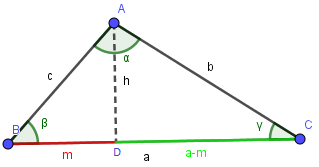
\includegraphics[width=0.50\linewidth]{secGD/figures/triangulo.png}
	\end{center}
	\caption{Triângulo para ilustrar a lei dos cossenos.}
	\label{fig:coslaw}
\end{figure}
\begin{itemize}
	\item \textbf{Demonstração Leis dos Cossenos:}
	
	Dado um triângulo qualquer, traça-se uma altura relativa ao lado $a$. Aplicando o \textit{Teorema de Pitágoras} no $\Delta ABD$:
	
	\begin{equation}
	c^{2}=m^{2}+h^{2} \rightarrow h^{2}=c^{2}-m^{2}
	\label{eq:tri1}
	\end{equation}
	
	Aplicando novamente \textit{Pitágoras}, porém, em $\Delta ADC$, obtemos:
	\begin{equation}
	b^{2}=h^{2}+(a-m)^{2}
	\label{eq:tri2}
	\end{equation}
	Substituindo na equação ~\ref{eq:tri2} o valor de $h^{2}$ obtido em ~\ref{eq:tri1}:
	$$
	b^{2}=c^{2}-m^{2}+a^{2}-2am+m^{2}
	$$
	$$
	b^{2}=c^{2}+a^{2}-2am
	$$
	Analisando a 
	Figura ~\ref{fig:coslaw}, pode-se perceber que $\frac{m}{c}=\cos\beta$, então:
	$$
	b^{2}=c^{2}+a^{2}-2ac\cos\beta
	$$
	Analogamente, obtém-se:
	$$
	c^{2}=a^{2}+b^{2}-2ab\cos\gamma
	$$
	$$
	a^{2}=b^{2}+c^{2}-2bc\cos\alpha
	$$
	Note também que se o argumento dos cossenos for $\frac{\pi}{2}$ recaímos no Teorema de Pitágoras. $\hfill\blacksquare$
	\item \textbf{Ângulos Entre 2 Vetores:}
	
	Sejam dois vetores $\overrightarrow{u}$ e $\overrightarrow{v} \in \mathbb{R}^2$, representados na Figura ~\ref{fig:diffbtvet}
	\begin{figure}[H]
		\begin{center}
			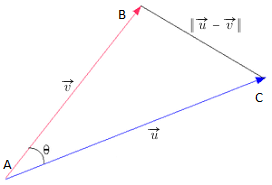
\includegraphics[width=0.4\linewidth]{secGD/figures/Angulovetoresnovo.png}
		\end{center}
		\caption{Diferença entre vetores $u$ e $v$}
		\label{fig:diffbtvet}
	\end{figure}
	Para encontrarmos o angulo $\theta$ utilizaremos a lei dos cossenos aplicada a $\Delta ABC$:
	\begin{equation}
	\|\overrightarrow{u}-\overrightarrow{v}\|^{2}=\|\overrightarrow{u}\|^{2} + \|\overrightarrow{v}\|^{2} - 2\|\overrightarrow{u}\|\|\overrightarrow{v}\|\cos\theta
	\label{eq:ang1}
	\end{equation}
	Utilizando a definição do produto escalar \cite{GASteinbruch}
	\begin{equation}
	\|\overrightarrow{u}-\overrightarrow{v}\|^{2}=\|\overrightarrow{u}\|^{2} + \|\overrightarrow{v}\|^{2} - 2\overrightarrow{u}\overrightarrow{v}
	\label{eq:ang2}
	\end{equation}
	Comparando a equação ~\ref{eq:ang1} com a ~\ref{eq:ang2}, obtemos trivialmente
	$$
	\|\overrightarrow{u}\|^{2} + \|\overrightarrow{v}\|^{2} - 2\|\overrightarrow{u}\|\|\overrightarrow{v}\|\cos\theta = \|\overrightarrow{u}\|^{2} + \|\overrightarrow{v}\|^{2} - 2\overrightarrow{u}\overrightarrow{v}
	$$
	$$
	\overrightarrow{u}\overrightarrow{v} = \|\overrightarrow{u}\|\|\overrightarrow{v}\|\cos\theta
	$$
	Logo,
	$$
	\cos\theta = \frac{\overrightarrow{u}\overrightarrow{v}}{\|\overrightarrow{u}\|\|\overrightarrow{v}\|} 
	$$
	$\hfill\blacksquare$
\end{itemize}